\documentclass[a4paper]{article}
\usepackage[utf8]{inputenc}
\usepackage[russian,english]{babel}
\usepackage[T2A]{fontenc}
\usepackage[left=10mm, top=20mm, right=18mm, bottom=15mm, footskip=10mm]{geometry}
\usepackage{indentfirst}
\usepackage{amsmath,amssymb}
\usepackage{mathastext} 
\usepackage[italicdiff]{physics}
\usepackage{graphicx}
\usepackage{caption}
\usepackage{float}
\usepackage{caption}
\renewcommand{\thefootnote}{\fnsymbol{footnote}}
\usepackage{tablefootnote}
\usepackage{footmisc}
\usepackage{textcomp}
\usepackage{multicol}
\usepackage{multirow}
\usepackage[parfill]{parskip}
\usepackage{makecell}
\usepackage{array}  
\usepackage{siunitx}
\usepackage{booktabs}
\sisetup{
    exponent-product = \cdot,
    per-mode = symbol,
    separate-uncertainty = true,
    uncertainty-separator = \,
}
\renewcommand\cellalign{cc} 
\renewcommand\cellgape{\Gape[2pt]} 
\usepackage[utf8]{inputenc}\newcommand{\approxtext}[1]{\ensuremath{\stackrel{\text{#1}}{\approx}}}
\usepackage[colorlinks=true, urlcolor=blue, linkcolor=blue, citecolor=blue]{hyperref}
\graphicspath{{images/}}
\DeclareGraphicsExtensions{.pdf,.png,.jpg}
\usepackage{wrapfig}
\captionsetup{labelformat=empty}
\usepackage{caption}
\captionsetup[figure]{name=Рисунок}
\captionsetup[table]{name=Таблица}
%\usepackage{newtxtext,newtxmath} 
\title{\textbf{Отчет о выполнении лабораторной работы 3.5.1}}
\date{}
\author{Котляров Михаил, Б01-402}

\begin{document}

\maketitle
	
\section{Введение}

\subsection{Цель работы}
Целью данной лабораторной работы является экспериментальное исследование параметров плазмы тлеющего газового разряда в неоне методом двойного зонда. В ходе работы измеряются вольт-амперная характеристика разряда и зондовые характеристики при различных токах разряда. На основе полученных данных определяются основные параметры плазмы: температура и концентрация электронов, степень ионизации, дебаевский радиус экранирования и плазменная частота.

\subsection{Оборудование}
Для выполнения работы используется следующее оборудование:
\begin{itemize}
\item стеклянная газоразрядная трубка, заполненная изотопом неона $^{22}\mathrm{Ne}$ при давлении 2~торр;
    \item катод — холодный (ненагреваемый) полый катод;
    \item три анода (Анод-I, Анод-II, Анод-III), где Анод-III в данной работе не используется;
    \item геттерный узел — стеклянный баллон с газопоглощающей плёнкой;
    \item высоковольтный источник питания (ВИП) с регулируемым выходным напряжением до 5~кВ;
    \item источник постоянного тока Б5-47 (0--30~В);
    \item балластный резистор $R_6 \approx 450$~кОм;
    \item высокоомный делитель напряжения ($R_1 + R_2)/R_2 = 10$, сопротивление $R_2 = 25$~МОм;
    \item двойной зонд из молибденовой проволоки диаметром $d = 0.2$~мм и длиной $l = 5.2$~мм;
    \item потенциометр $R$ для регулировки напряжения на зондах;
    \item переключатель полярности П2;
    \item дискретный переключатель «V» для выбора выходного напряжения источника питания GPS;
    \item цифровые мультиметры GDM: $V_1$ — для измерения падения напряжения на трубке, $V_2$ — для измерения напряжения на зондах;
    \item миллиамперметры: $A_1$ — для измерения тока разряда, $A_2$ — для измерения зондового тока.
\end{itemize}
\subsection{Теоретические сведения}
Плазма — это ионизованный газ, в котором концентрации положительных и отрицательных зарядов практически равны (квазинейтральность), а поведение частиц носит коллективный характер. Основными параметрами плазмы являются:
\begin{itemize}
\item \textbf{Температура электронов} $T_e$, обычно выражаемая в энергетических единицах (эВ): $1~\text{эВ} \approx 11\,600~\text{К}$;
    \item \textbf{Концентрация электронов} $n_e$ (и ионов $n_i$, при $Z=1$ предполагается $n_e = n_i$);
    \item \textbf{Плазменная частота} — характерная частота собственных колебаний электронов:
    \[
        \omega_p = \sqrt{\frac{4\pi n_e e^2}{m_e}},
    \]
    где $e$ — заряд электрона, $m_e$ — его масса;
    \item \textbf{Дебаевский радиус экранирования} — характерный масштаб, на котором нарушается квазинейтральность:
    \[
        r_D = \sqrt{\frac{k_\text{Б} T_e}{4\pi n_e e^2}}.
    \]
    В случае $T_e \gg T_i$ (неравновесная плазма) используется электронная поляризационная длина $r_{De}$, определяемая той же формулой с $T = T_e$;
    \item \textbf{Степень ионизации} $\alpha = n_e / n_0$, где $n_0$ — концентрация нейтральных частиц, связанная с давлением $P$ идеально-газовым соотношением $P = n_0 k_\text{Б} T_g$.

Когда в плазму помещается зонд, не подключённый к внешней цепи (плавающий зонд), он заряжается до определённого потенциала $U_f$, называемого \textbf{плавающим потенциалом}. Этот потенциал определяется условием равенства токов электронов и ионов на зонд, так как в равновесии суммарный ток на зонд должен быть равен нулю. Плавающий потенциал обычно отрицателен по сравнению с потенциалом плазмы, так как электроны, обладающие большей подвижностью, приходят на зонд быстрее, чем ионы, и зонд заряжается отрицательно до тех пор, пока не установится баланс токов.

Для диагностики плазмы применяется \textbf{двойной зонд} — пара одинаковых электродов, погружённых в плазму. При малых напряжениях между зондами ($|U| \ll |U_f|$, где $U_f$ — плавающий потенциал) вольт-амперная характеристика описывается выражением:
\[
    I(U) = I_{i\text{н}} \tanh\!\left(\frac{eU}{2k_\text{Б} T_e}\right),
\]
где $I_{i\text{н}}$ — ионный ток насыщения. Из наклона характеристики в начале координат определяется температура электронов:
\[
    k_\text{Б} T_e = \frac{1}{2} \frac{e I_{i\text{н}}}{\left.\frac{dI}{dU}\right|_{U=0}}.
\]
Концентрация электронов вычисляется по полуэмпирической формуле Бома:
\[
    I_{i\text{н}} \approx 0{,}4\, n_e e S \sqrt{\frac{2 k_\text{Б} T_e}{m_i}},
\]
где $S \approx \pi d l$ — площадь поверхности зонда, $m_i$ — масса иона.
\end{itemize}
\subsection*{Экспериментальная установка}
Экспериментальная установка состоит из стеклянной газоразрядной трубки, заполненной неоном при давлении $P = 2$~мм рт. ст. Разряд возбуждается между катодом и одним из анодов. При изучении вольт-амперной характеристики разряда используется Анод-I, подключаемый через балластный резистор $R_6$ к ВИП. Напряжение на трубке измеряется вольтметром $V_1$ через высокоомный делитель напряжения, а ток разряда — амперметром $A_1$. 

\clearpage
\begin{figure}[h]
        \center{
\includegraphics[width=0.81\textwidth]{Pictures/ustanovka.png}}
        \caption{Рисунок 1. Экспериментальная установка}
\end{figure}

При зондовых измерениях используется Анод-II, в пространстве между которым и катодом расположен двойной зонд. Зонды изготовлены из молибденовой проволоки ($d = 0.2$~мм, $l = 5.2$~мм). Напряжение на зондах регулируется потенциометром $R$ и измеряется вольтметром $V_2$, а ток через зонды — микроамперметром $A_2$. Переключатель П2 позволяет изменять полярность напряжения на зондах. Все измерения проводятся при фиксированных значениях тока разряда $I_p$, контролируемого амперметром $A_1$.

\section{Выполнение}

\subsection{Измерение вольт-амперной характеристики разряда}

\begin{enumerate}
\item \textbf{Подготовка схемы:}

     Установим переключатель П1 в положение «Анод-I». Подготовим приборы: вольтметр $V_1$ (для измерения напряжения на трубке) и амперметр $A_1$ (для измерения тока разряда).

\textbf{Определение напряжения зажигания:}
    \item Плавно увеличивая выходное напряжение ВИП, следим за показаниями вольтметра $V_1$.
        \item Запишем значение напряжения $U_{\text{заж}}$, которое показывает вольтметр $V_1$ непосредственно перед зажиганием разряда (резкое увеличение тока $I_p$). $U_{\text{заж}} = 1940$ В.

\textbf{Снятие основной ветви ВАХ:}
    \item Установим минимальное напряжение ВИП.
        \item Постепенно увеличивая напряжение ВИП, снимаем показания вольтметра $V_1$ (напряжение $U_p$) и амперметра $A_1$ (ток $I_p$) в диапазоне токов от 0,5 мА до 5 мА. Измерения проведем как при нарастании, так и при убывании тока.
\clearpage
\begin{table}[h!]
    \centering
    \begin{minipage}{0.48\textwidth}
        \centering
        
        \label{tab:vac_increase}
        \begin{tabular}{|c|c|}
            \hline
            $U_p$, В & $I_p$, мА \\ \hline
            340,2 & 0,516 \\ \hline
            337,0 & 0,598 \\ \hline
            332,5 & 0,683 \\ \hline
            330,0 & 0,762 \\ \hline
            327,8 & 0,821 \\ \hline
            324,8 & 0,916 \\ \hline
            321,0 & 1,065 \\ \hline
            318,0 & 1,215 \\ \hline
            316,1 & 1,325 \\ \hline
            314,0 & 1,472 \\ \hline
            308,0 & 1,784 \\ \hline
            299,0 & 1,972 \\ \hline
            287,0 & 2,106 \\ \hline
            280,0 & 2,202 \\ \hline
            264,0 & 2,604 \\ \hline
            251,0 & 2,906 \\ \hline
            247,0 & 3,014 \\ \hline
            238,0 & 3,197 \\ \hline
            230,0 & 3,550 \\ \hline
            225,0 & 4,252 \\ \hline
            217,0 & 5,017 \\ \hline
        \end{tabular}
\caption{Таблица 1.1. ВАХ разряда при повышении тока $I_p$.}
    \end{minipage}
    \hfill
    \begin{minipage}{0.48\textwidth}
        \centering

        \label{tab:vac_decrease}
        \begin{tabular}{|c|c|}
            \hline
            $U_p$, В & $I_p$, мА \\ \hline
            217,0 & 4,969 \\ \hline
            221,0 & 4,564 \\ \hline
            223,8 & 4,168 \\ \hline
            224,8 & 3,781 \\ \hline
            230,7 & 3,396 \\ \hline
            247,0 & 2,991 \\ \hline
            254,0 & 2,822 \\ \hline
            263,0 & 2,637 \\ \hline
            280,0 & 2,232 \\ \hline
            286,0 & 2,121 \\ \hline
            295,0 & 1,993 \\ \hline
            306,8 & 1,805 \\ \hline
            313,0 & 1,502 \\ \hline
            319,0 & 1,129 \\ \hline
            328,0 & 0,802 \\ \hline
            336,7 & 0,599 \\ \hline
            341,0 & 0,531 \\ \hline
        \end{tabular}
        \caption{Таблица 1.2. ВАХ разряда при понижении тока $I_p$.}
    \end{minipage}
\end{table}

Построим график ВАХ аппроксимируя его сплайном 3-й степени и найдем максимальное дифференциальное сопротивление $\frac{dU}{dI}$.
\begin{figure}[h]
        \center{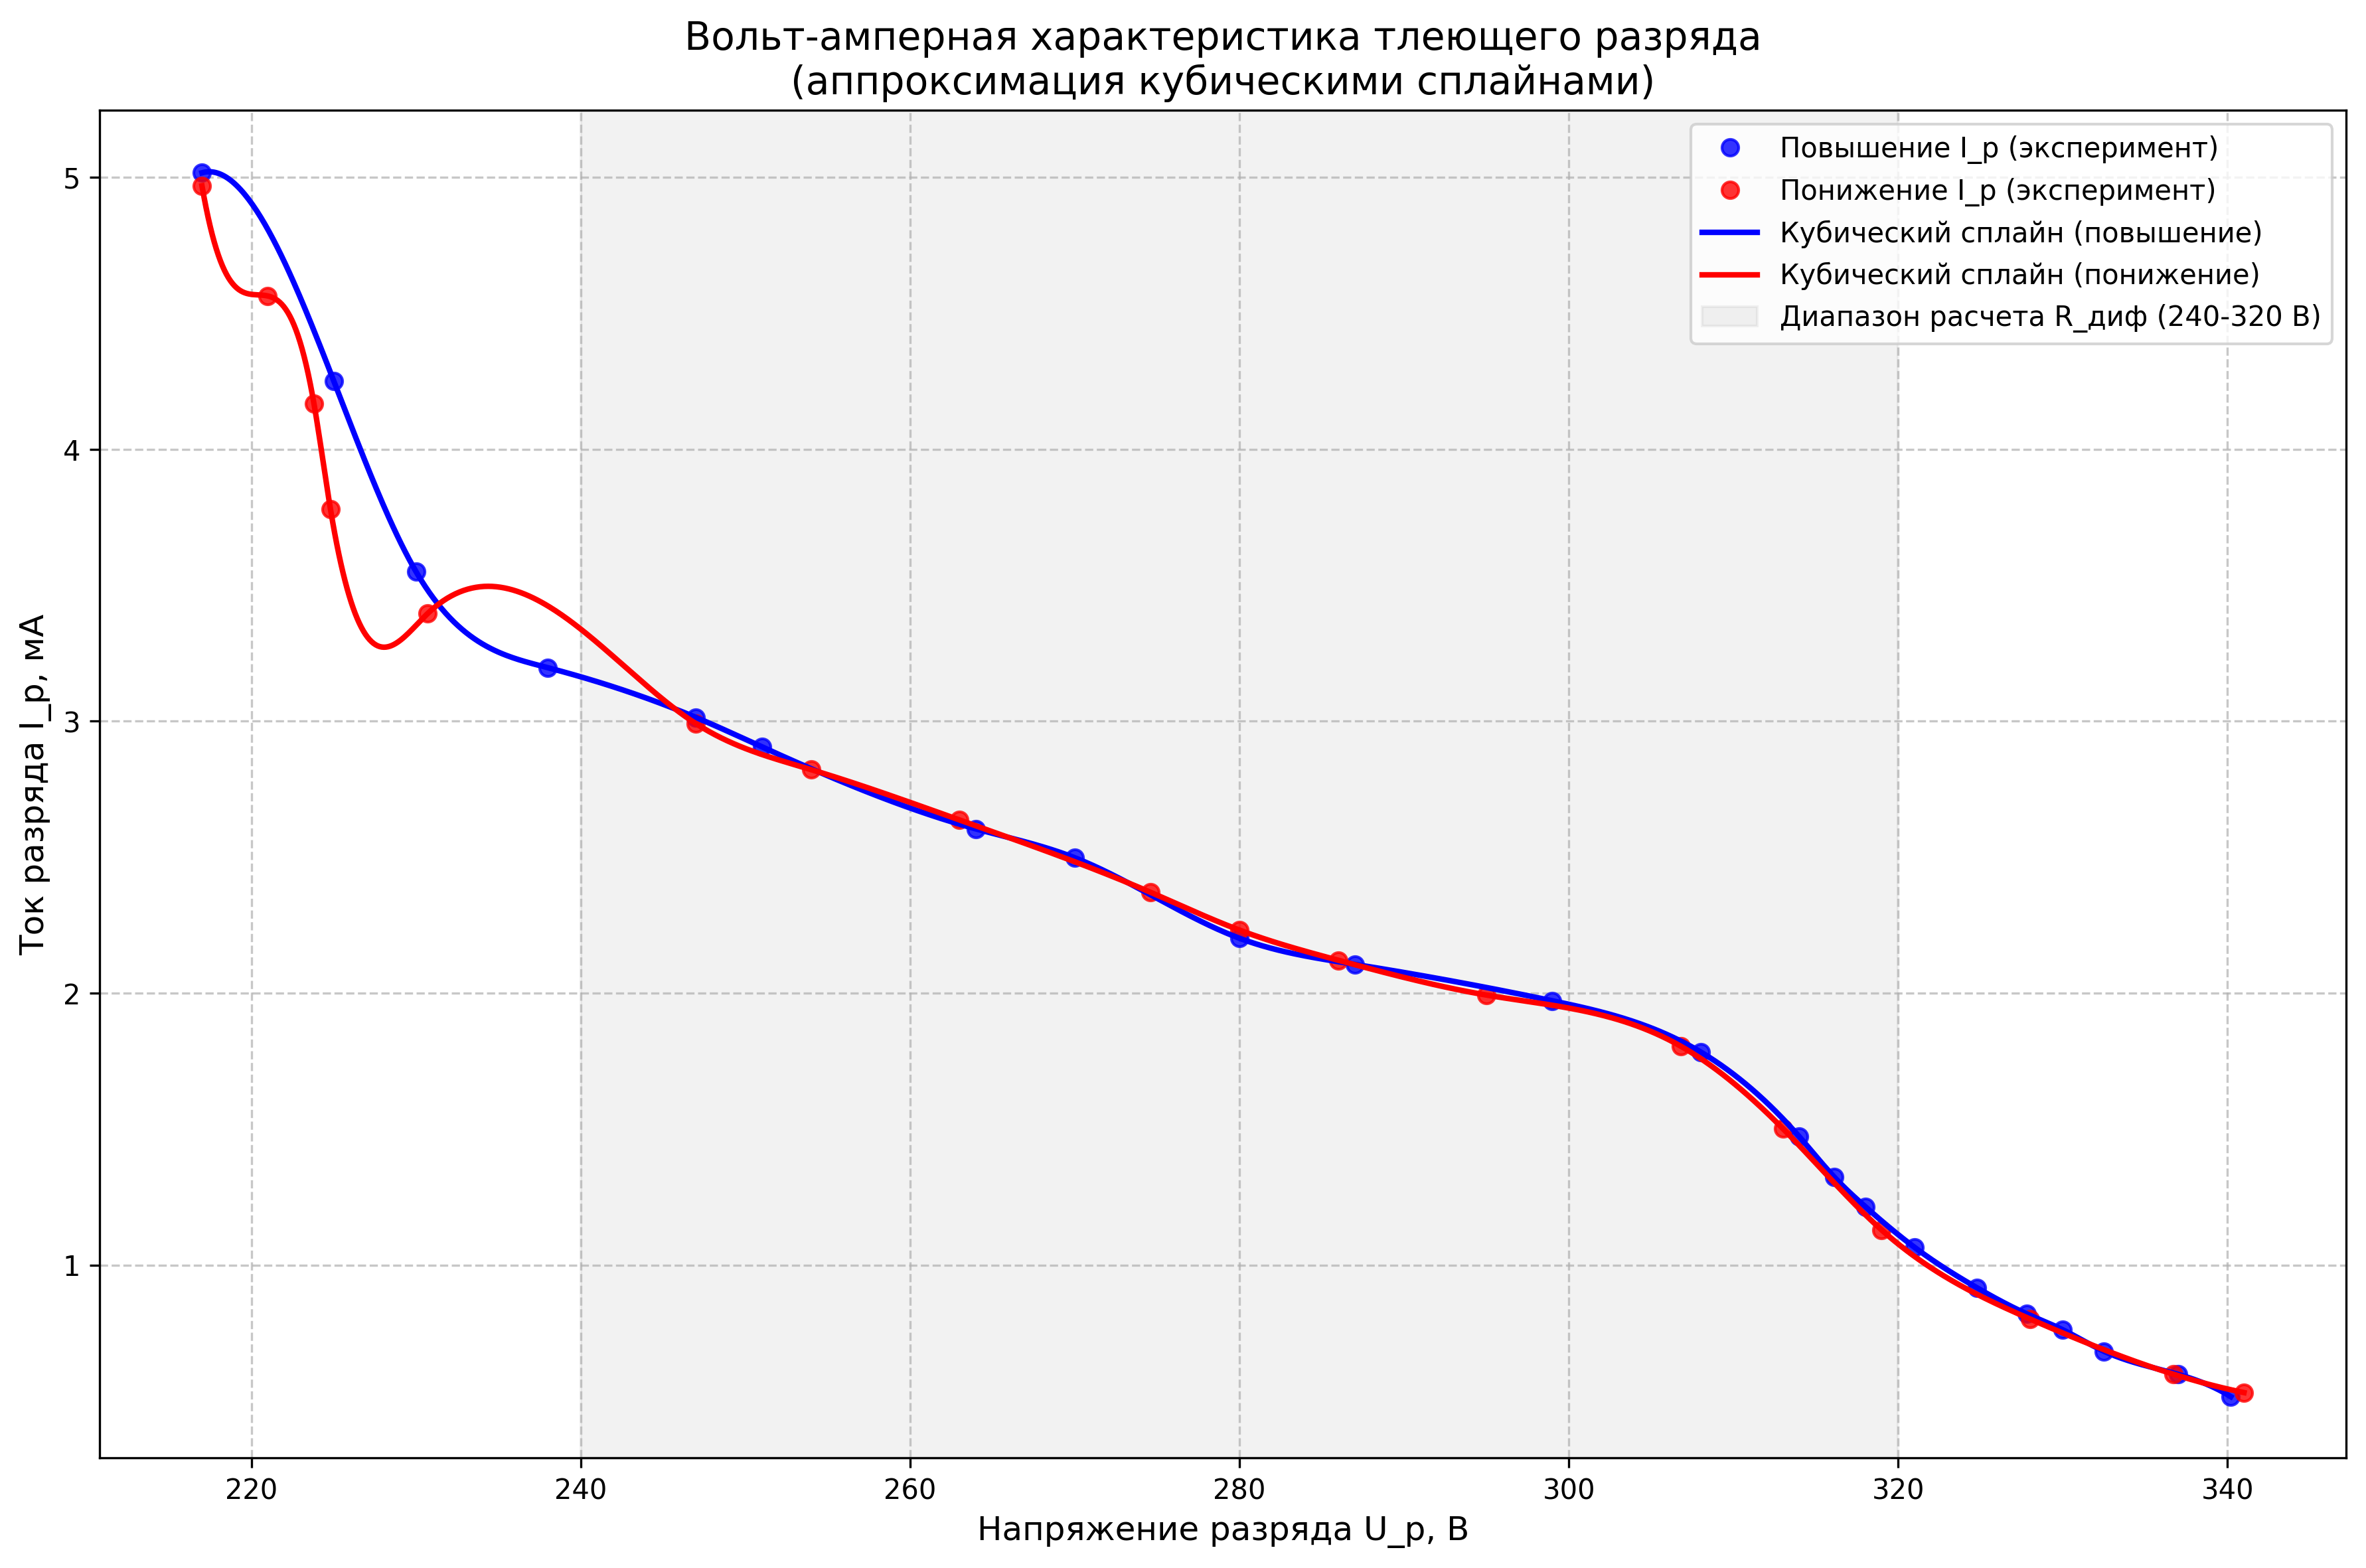
\includegraphics[width=0.7\textwidth]{Graphics/VA_characteristic_cubic_spline.png}}
        \caption{График 1. ВАХ тлеющего разряда}
\end{figure}

Мы искали дифференециальное сопротивление по двум методам - с помощью аппроксимации сплайном и с помощью метода конечных приращений. Затем взяли среднее значение: $R_{\text{диф}}^{\text{сплайн}} = 107,7 \pm 3,3$ кОм ($\varepsilon_{R_{\text{диф}}^{\text{сплайн}}} = 3,06 \%$), $R_{\text{диф}}^{\text{конеч}} = 79,9 \pm 13,4$ кОм ($\varepsilon_{R_{\text{диф}}^{\text{конеч}}} = 16,77 \%$), $R_{\text{диф}}^{\text{ср}} = 93,8$ кОм, \\$\sigma_{R_{\text{диф}}^{\text{ср}}} = \frac{1}{2} \sqrt{\left(\sigma_{R_{\text{диф}}^{\text{сплайн}}} \right)^2 + \left( \sigma_{R_{\text{диф}}^{\text{конеч}}} \right)^2 } = 6,9$ кОм ($\varepsilon_{R_{\text{диф}}^{\text{ср}}} = 7,36 \%$).

\subsection{Измерение зондовых характеристик}

    \item Уменьшим напряжение ВИП до нуля. Переведём переключатель П1 в положение «Анод-II». Теперь разряд будет происходить между катодом и Анодом-II, где находится двойной зонд.  Подготовим приборы: переключатель полярности П2, вольтметр $V_2$ (для измерения напряжения на зондах) и микроамперметр $A_2$ (для измерения зондового тока).

    \item Плавно увеличиваем напряжение ВИП до возникновения разряда. Установим максимальное значение разрядного тока $I_p = 5$ мА, как указано в техническом описании.

    \item Подготовим к работе источник питания зондов. С помощью потенциометра $R$ установим на зонде максимальное напряжение $U^{\text{max}}_{\text{з}} = 25$ В, как указано в описании.

    \item Измерим вольт-амперную характеристику двойного зонда $I_{\text{з}}(U_{\text{з}})$ в диапазоне от $-U^{\text{max}}_{\text{з}}$ до $+U^{\text{max}}_{\text{з}}$. В процессе измерений следим, чтобы ток разряда $I_p$ оставался постоянным. При достижении тока $I_{\text{з}} = 0$ переключим полярность подключения зонда с помощью переключателя П2 и продолжим измерения. Одновременно строим приближенный график $I(U)$ в тетради, чтобы убедиться в наличии асимптот.

    \item Повторим процедуру снятия зондовой характеристики при других значениях тока разряда $I_p$ (4 мА, 3.02 мА, 1.5 мА).

        \item Запишем параметры установки: давление в трубке (2 торр), геометрические размеры зондов ($d = 0.2$ мм, $l = 5.2$ мм).

\item Построим ВАХ двойного зонда для разных токов, аппроксимирую гиперболическим тангенсом согласно теории. Касательные в нуле проведем по аппроксимации и по методу конечных приращений. Асимптоты на краях проведем по методу конечных приращений и как касательные к аппроксимации в крайних точках.

\begin{figure}[h]
        \center{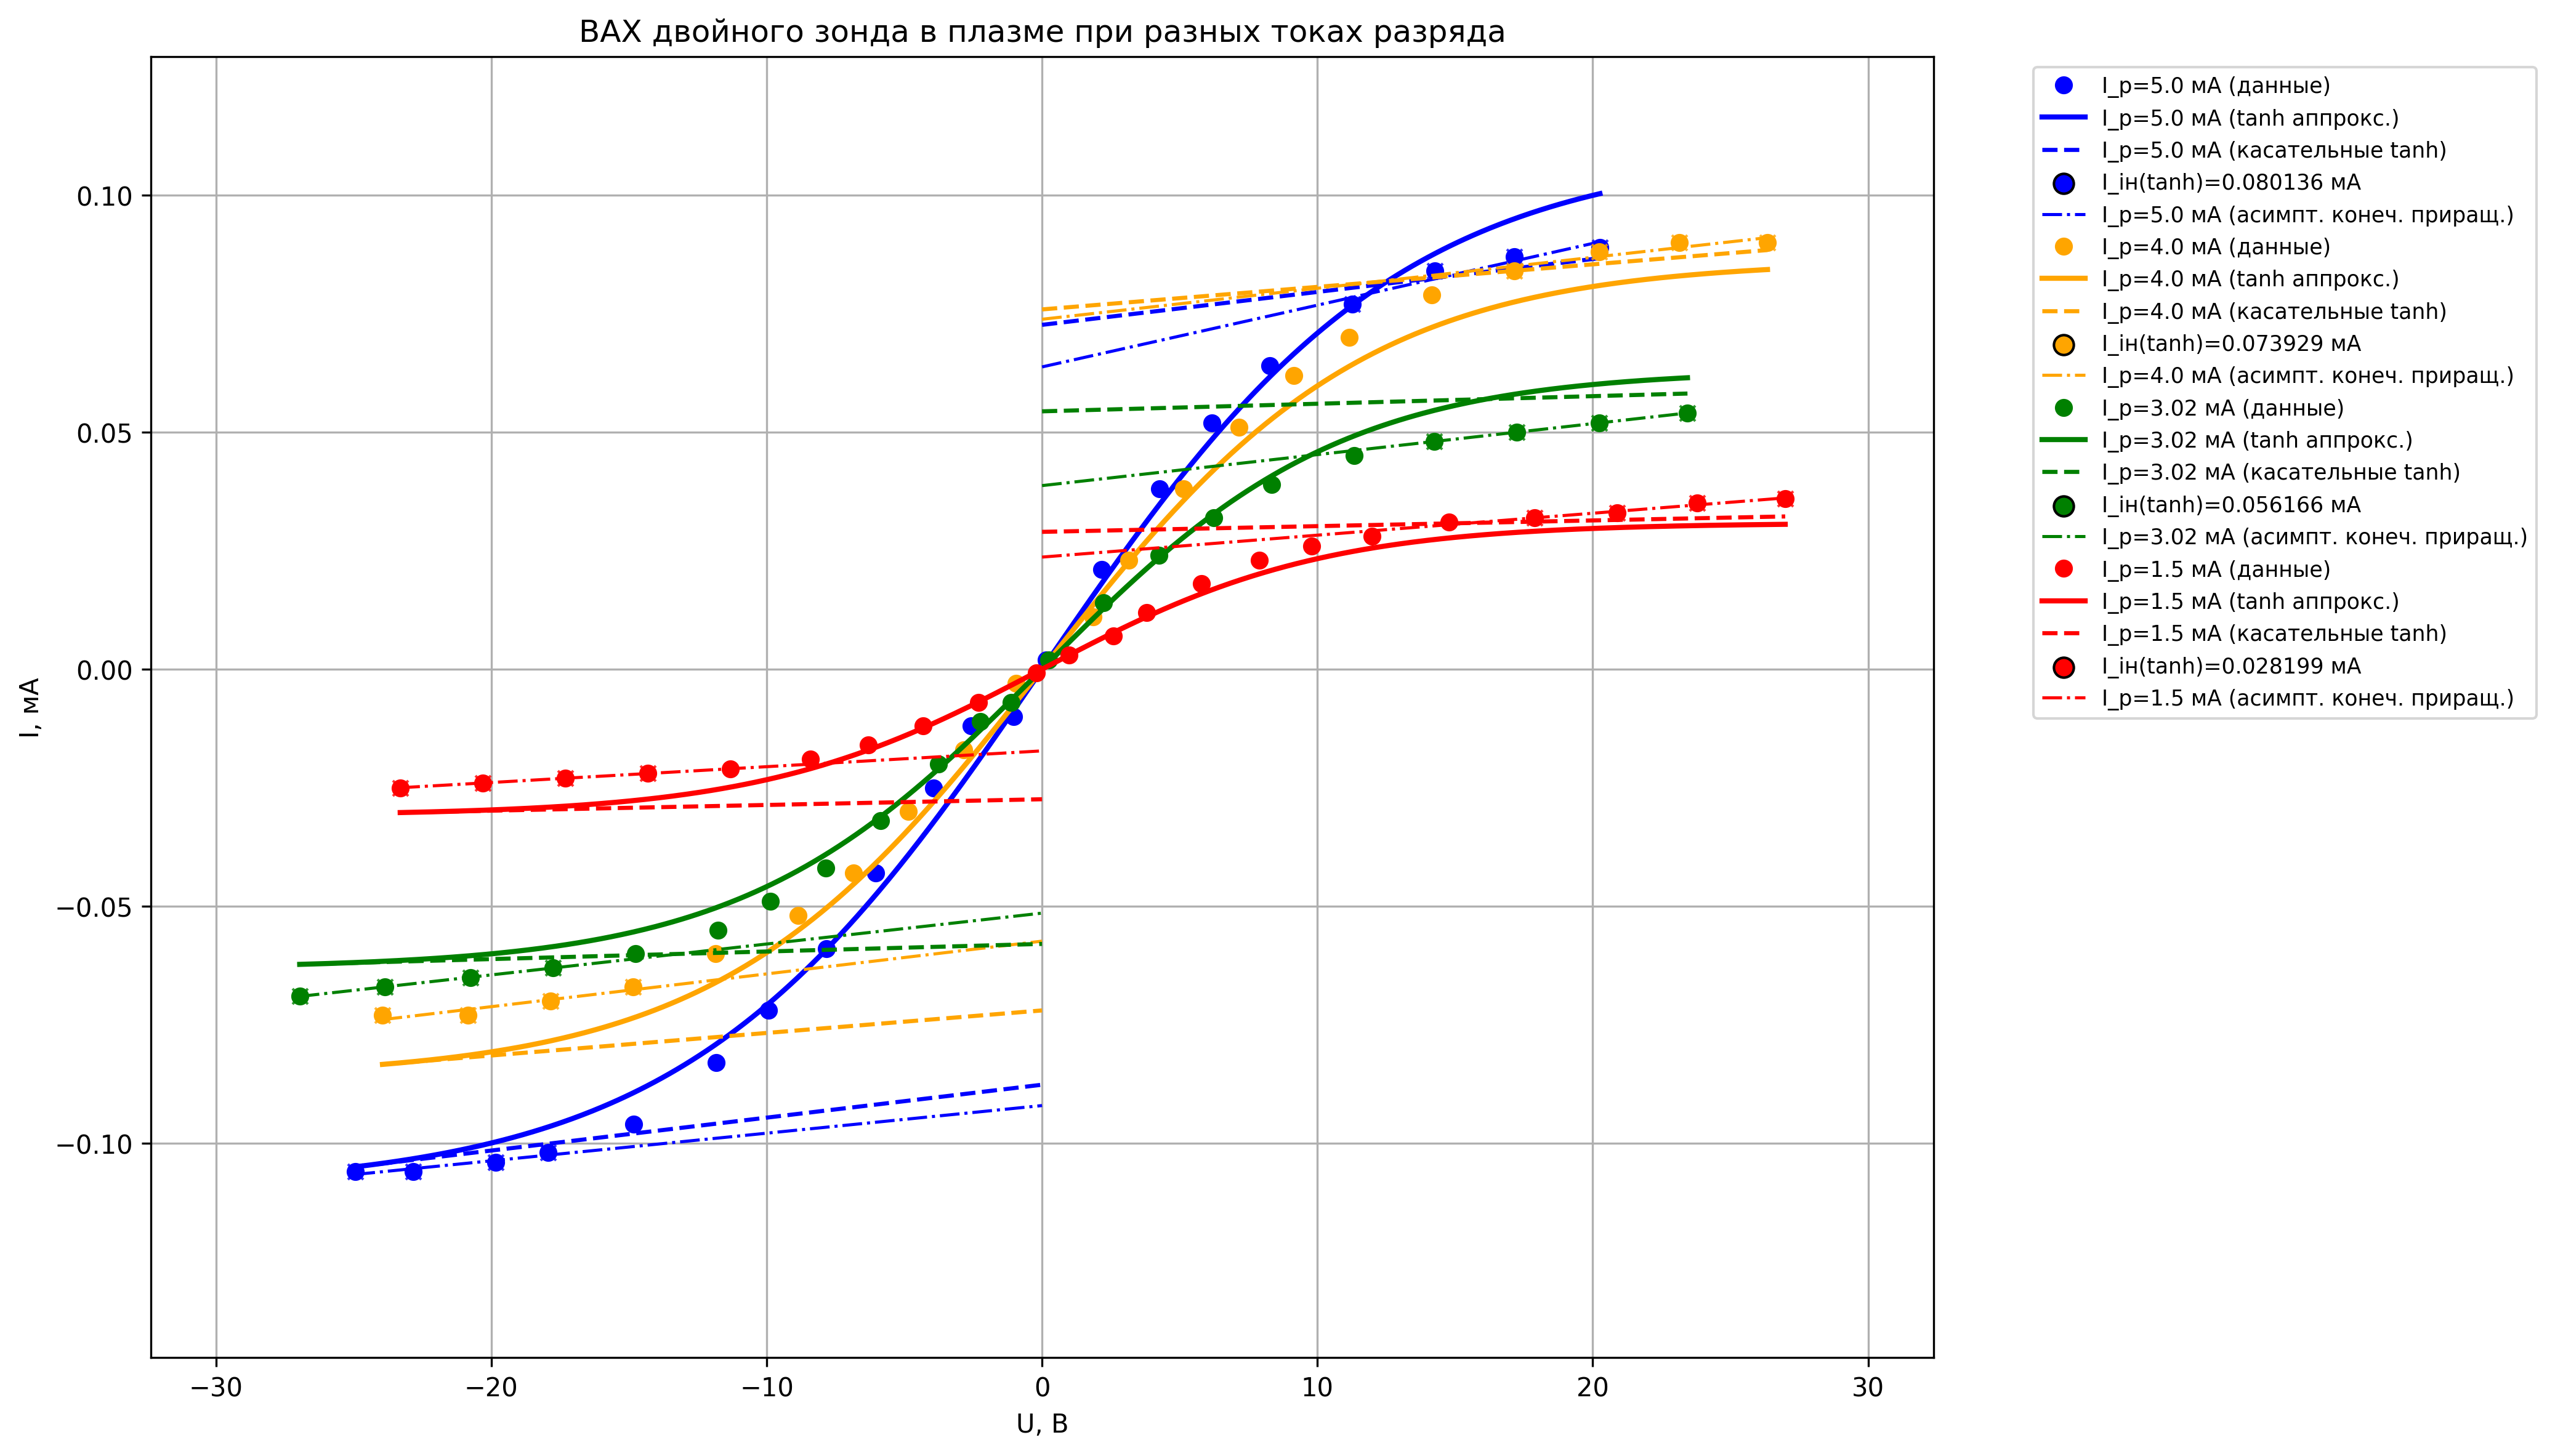
\includegraphics[width=1.05\textwidth]{Graphics/VA_zond.png}}
        \caption{График 2. ВАХ двойного зонда в плазме}
\end{figure}
\clearpage
\begin{table}[h!]
    \centering

    \label{tab:probe_data}
    \begin{tabular}{|c|c|c|c|c|}
        \hline
        \textbf{Ток разряда, мА} & \textbf{Метод} & $I_{i\text{н}} \pm \Delta I_{i\text{н}}$, мА & $dI/dU|_{U=0} \pm \Delta (dI/dU)$, мА/В \\
        \hline
        \multirow{3}{*}{5} & Сплайн & $0{,}0801 \pm 0{,}0027$ & $0{,}0084 \pm 0{,}0007$ \\
        \cline{2-4}
         & Конечные приращения & $0{,}0779 \pm 0{,}0027$ & $0{,}0078 \pm 0{,}0008$ \\
        \cline{2-4}
         & Усреднённое & $0{,}0790 \pm 0{,}0019$ & $0{,}0082 \pm 0{,}0005$ \\
        \hline
        \multirow{3}{*}{4} & Сплайн & $0{,}0739 \pm 0{,}0025$ & $0{,}0074 \pm 0{,}0007$ \\
        \cline{2-4}
         & Конечные приращения & $0{,}0656 \pm 0{,}0029$ & $0{,}0064 \pm 0{,}0003$ \\
        \cline{2-4}
         & Усреднённое & $0{,}0704 \pm 0{,}0019$ & $0{,}0065 \pm 0{,}0003$ \\
        \hline
        \multirow{3}{*}{3,02} & Сплайн & $0{,}0562 \pm 0{,}0017$ & $0{,}0058 \pm 0{,}0006$ \\
        \cline{2-4}
         & Конечные приращения & $0{,}0451 \pm 0{,}0001$ & $0{,}0056 \pm 0{,}0002$ \\
        \cline{2-4}
         & Усреднённое & $0{,}0451 \pm 0{,}0001$ & $0{,}0056 \pm 0{,}0002$ \\
        \hline
        \multirow{3}{*}{1,5} & Сплайн & $0{,}0282 \pm 0{,}0012$ & $0{,}0030 \pm 0{,}0005$ \\
        \cline{2-4}
         & Конечные приращения & $0{,}0204 \pm 0{,}0006$ & $0{,}0028 \pm 0{,}0001$ \\
        \cline{2-4}
         & Усреднённое & $0{,}0219 \pm 0{,}0005$ & $0{,}0028 \pm 0{,}0001$ \\
        \hline
    \end{tabular}
    \caption{Таблица 2. Результаты обработки зондовых характеристик при различных токах разряда.}
\end{table}

Средние значения брались как взвешенное по погрешностям среднее, т.е., например, для тока насыщения $I_{\text{iн}}^{\text{ср}} = \frac{w^{\text{конеч}} I_{\text{iн}}^{\text{конеч}} +w^{\text{сплайн}} I_{\text{iн}}^{\text{сплайн}}}{w^{\text{конеч}} + w^{\text{сплайн}}}$, $\Delta I_{\text{iн}}^{\text{ср}} = \sqrt{\frac{1}{w^{\text{конеч}} + w^{\text{сплайн}}}}$, $w = \frac{1}{\left(\Delta I_{\text{iн}} \right)^2}$.

\item рассчитаем теперь температуру электронов $T_e$, концентрацию электронов и ионов $n_i \approx n_e$, ленгмюровскую частоту $\omega_p$ электронов, дебаевский радиус электронов $r_{De}$и экранирования $r_D$, среднее число ионов в дебаевской сфере $N_D$, степень ионизации плазмы $\alpha$.

\begin{table}[h!]
\centering

\label{tab:plasma_params}
\begin{tabular}{|l|c|c|c|c|c|c|c|c|}
\hline
\multirow{2}{*}{Параметр} & 
\multicolumn{2}{c|}{$I_p = 5$~мА} & 
\multicolumn{2}{c|}{$I_p = 4$~мА} & 
\multicolumn{2}{c|}{$I_p = 3,02$~мА} & 
\multicolumn{2}{c|}{$I_p = 1,5$~мА} \\
\cline{2-9}
& Значение & $\varepsilon$, \% & Значение & $\varepsilon$, \% & Значение & $\varepsilon$, \% & Значение & $\varepsilon$, \% \\
\hline

\multirow{2}{*}{$T_e$, К} & \multirow{2}{*}{$55900 \pm 3843$} & \multirow{2}{*}{6,87} & \multirow{2}{*}{$62386 \pm 2990$} & \multirow{2}{*}{4,79} & \multirow{2}{*}{$46615 \pm 1621$} & \multirow{2}{*}{3,48} & \multirow{2}{*}{$45224 \pm 1474$} & \multirow{2}{*}{3,26} \\
& & & & & & & & \\
\cline{1-1} \cline{2-9}

$T_e$, эВ & $4,82 \pm 0,33$ & & $5,38 \pm 0,26$ & & $4,02 \pm 0,14$ & & $3,90 \pm 0,13$ & \\
\hline

$n_e = n_i$, $10^{10}$~см$^{-3}$ & $5,56 \pm 0,23$ & 4,21 & $4,69 \pm 0,17$ & 3,60 & $3,48 \pm 0,06$ & 1,75 & $1,71 \pm 0,05$ & 2,90 \\
\hline

$r_{De}$, $10^{-3}$~см & $6,92 \pm 0,28$ & 4,03 & $7,96 \pm 0,24$ & 3,00 & $7,99 \pm 0,16$ & 1,95 & $11,22 \pm 0,24$ & 2,18 \\
\hline

$r_D$, $10^{-4}$~см & $5,06 \pm 0,20$ & 4,03 & $5,51 \pm 0,17$ & 3,00 & $6,39 \pm 0,12$ & 1,95 & $9,10 \pm 0,20$ & 2,18 \\
\hline

$N_D$ & $30,1 \pm 3,9$ & 12,8 & $32,8 \pm 3,2$ & 9,68 & $38,0 \pm 2,3$ & 6,09 & $54,1 \pm 3,9$ & 7,16 \\
\hline

$\alpha$, $10^{-7}$ & $8,64 \pm 0,35$ & 4,03 & $7,28 \pm 0,22$ & 3,00 & $5,40 \pm 0,11$ & 1,95 & $2,66 \pm 0,06$ & 2,18 \\
\hline

$\omega_p$, $10^{10}$~рад/с & $1,330 \pm 0,028$ & 2,11 & $1,221 \pm 0,022$ & 1,80 & $1,052 \pm 0,009$ & 0,87 & $0,738 \pm 0,011$ & 1,45 \\
\hline

\end{tabular}
\caption{Таблица 3. Параметры плазмы при различных токах разряда}
\end{table}

\item Построим графики $T_e(I_\text{р})$ и $n_e(I_\text{р})$.

\begin{figure}[h]
        \center{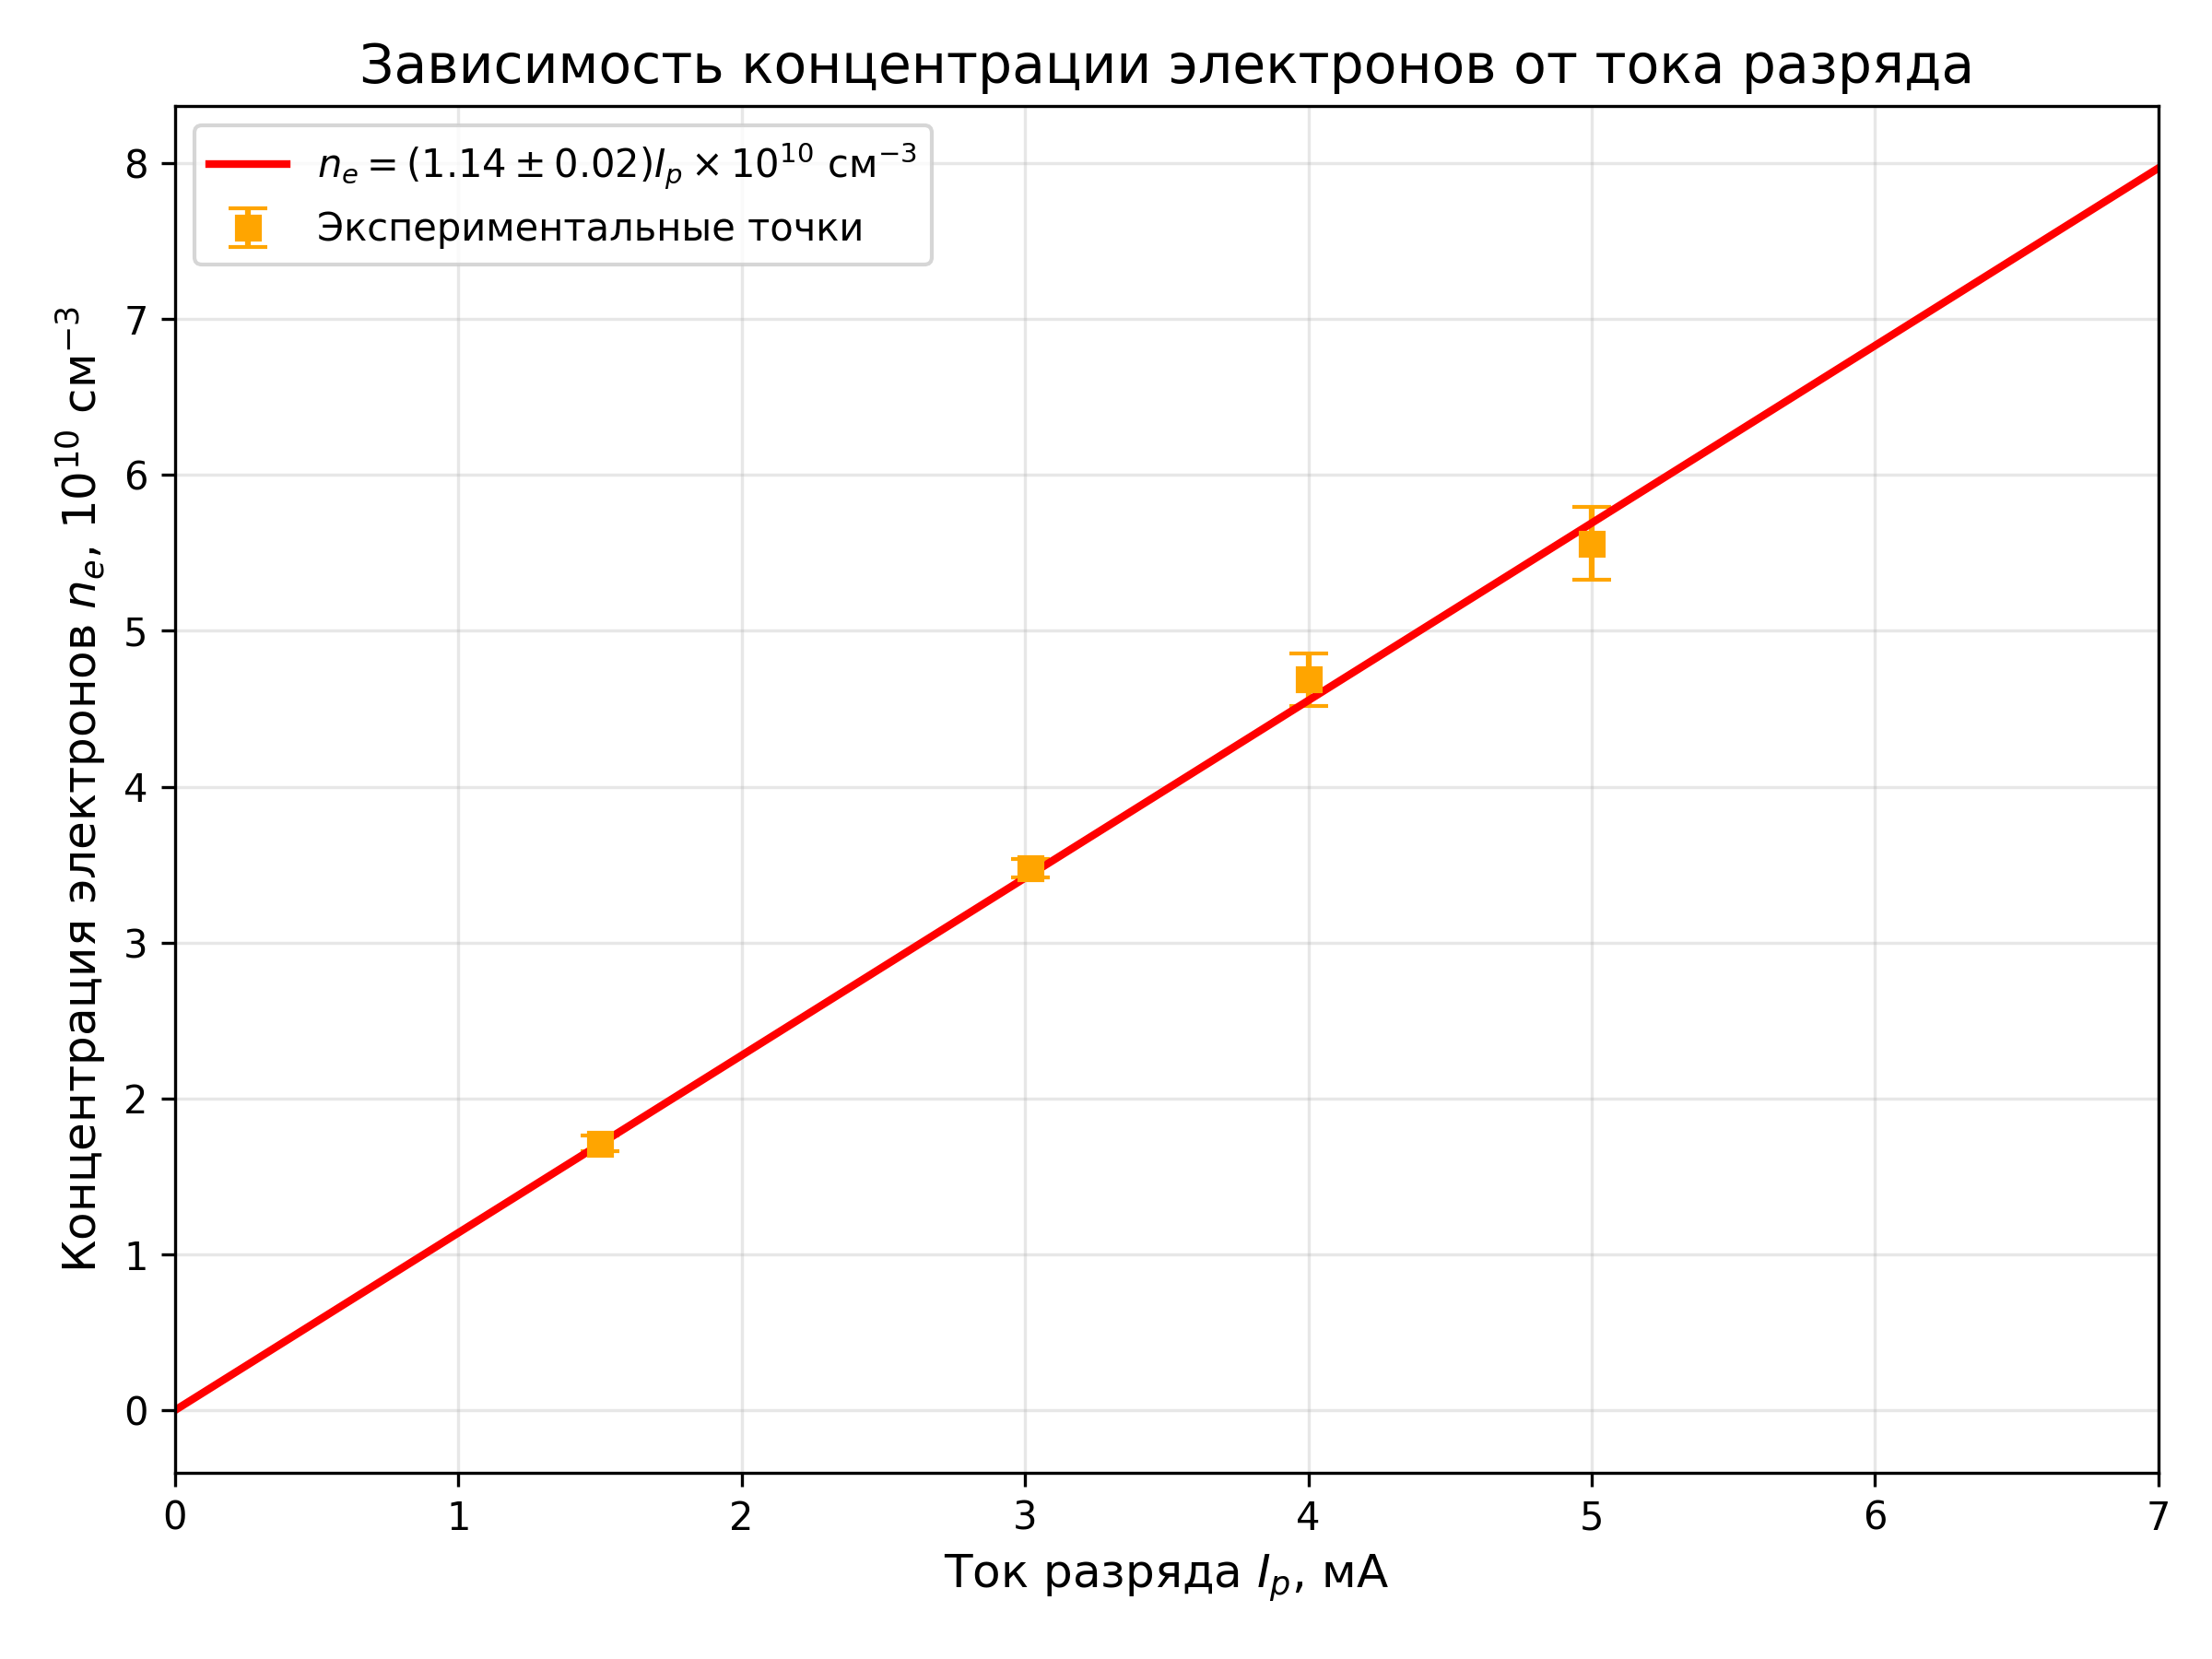
\includegraphics[width=0.7\textwidth]{Graphics/ne_vs_Ip_linear_fit.png}}
        \caption{График 3. Зависимость концентрации электронов от тока разряда в плазме}
\end{figure}

\begin{figure}[h]
        \center{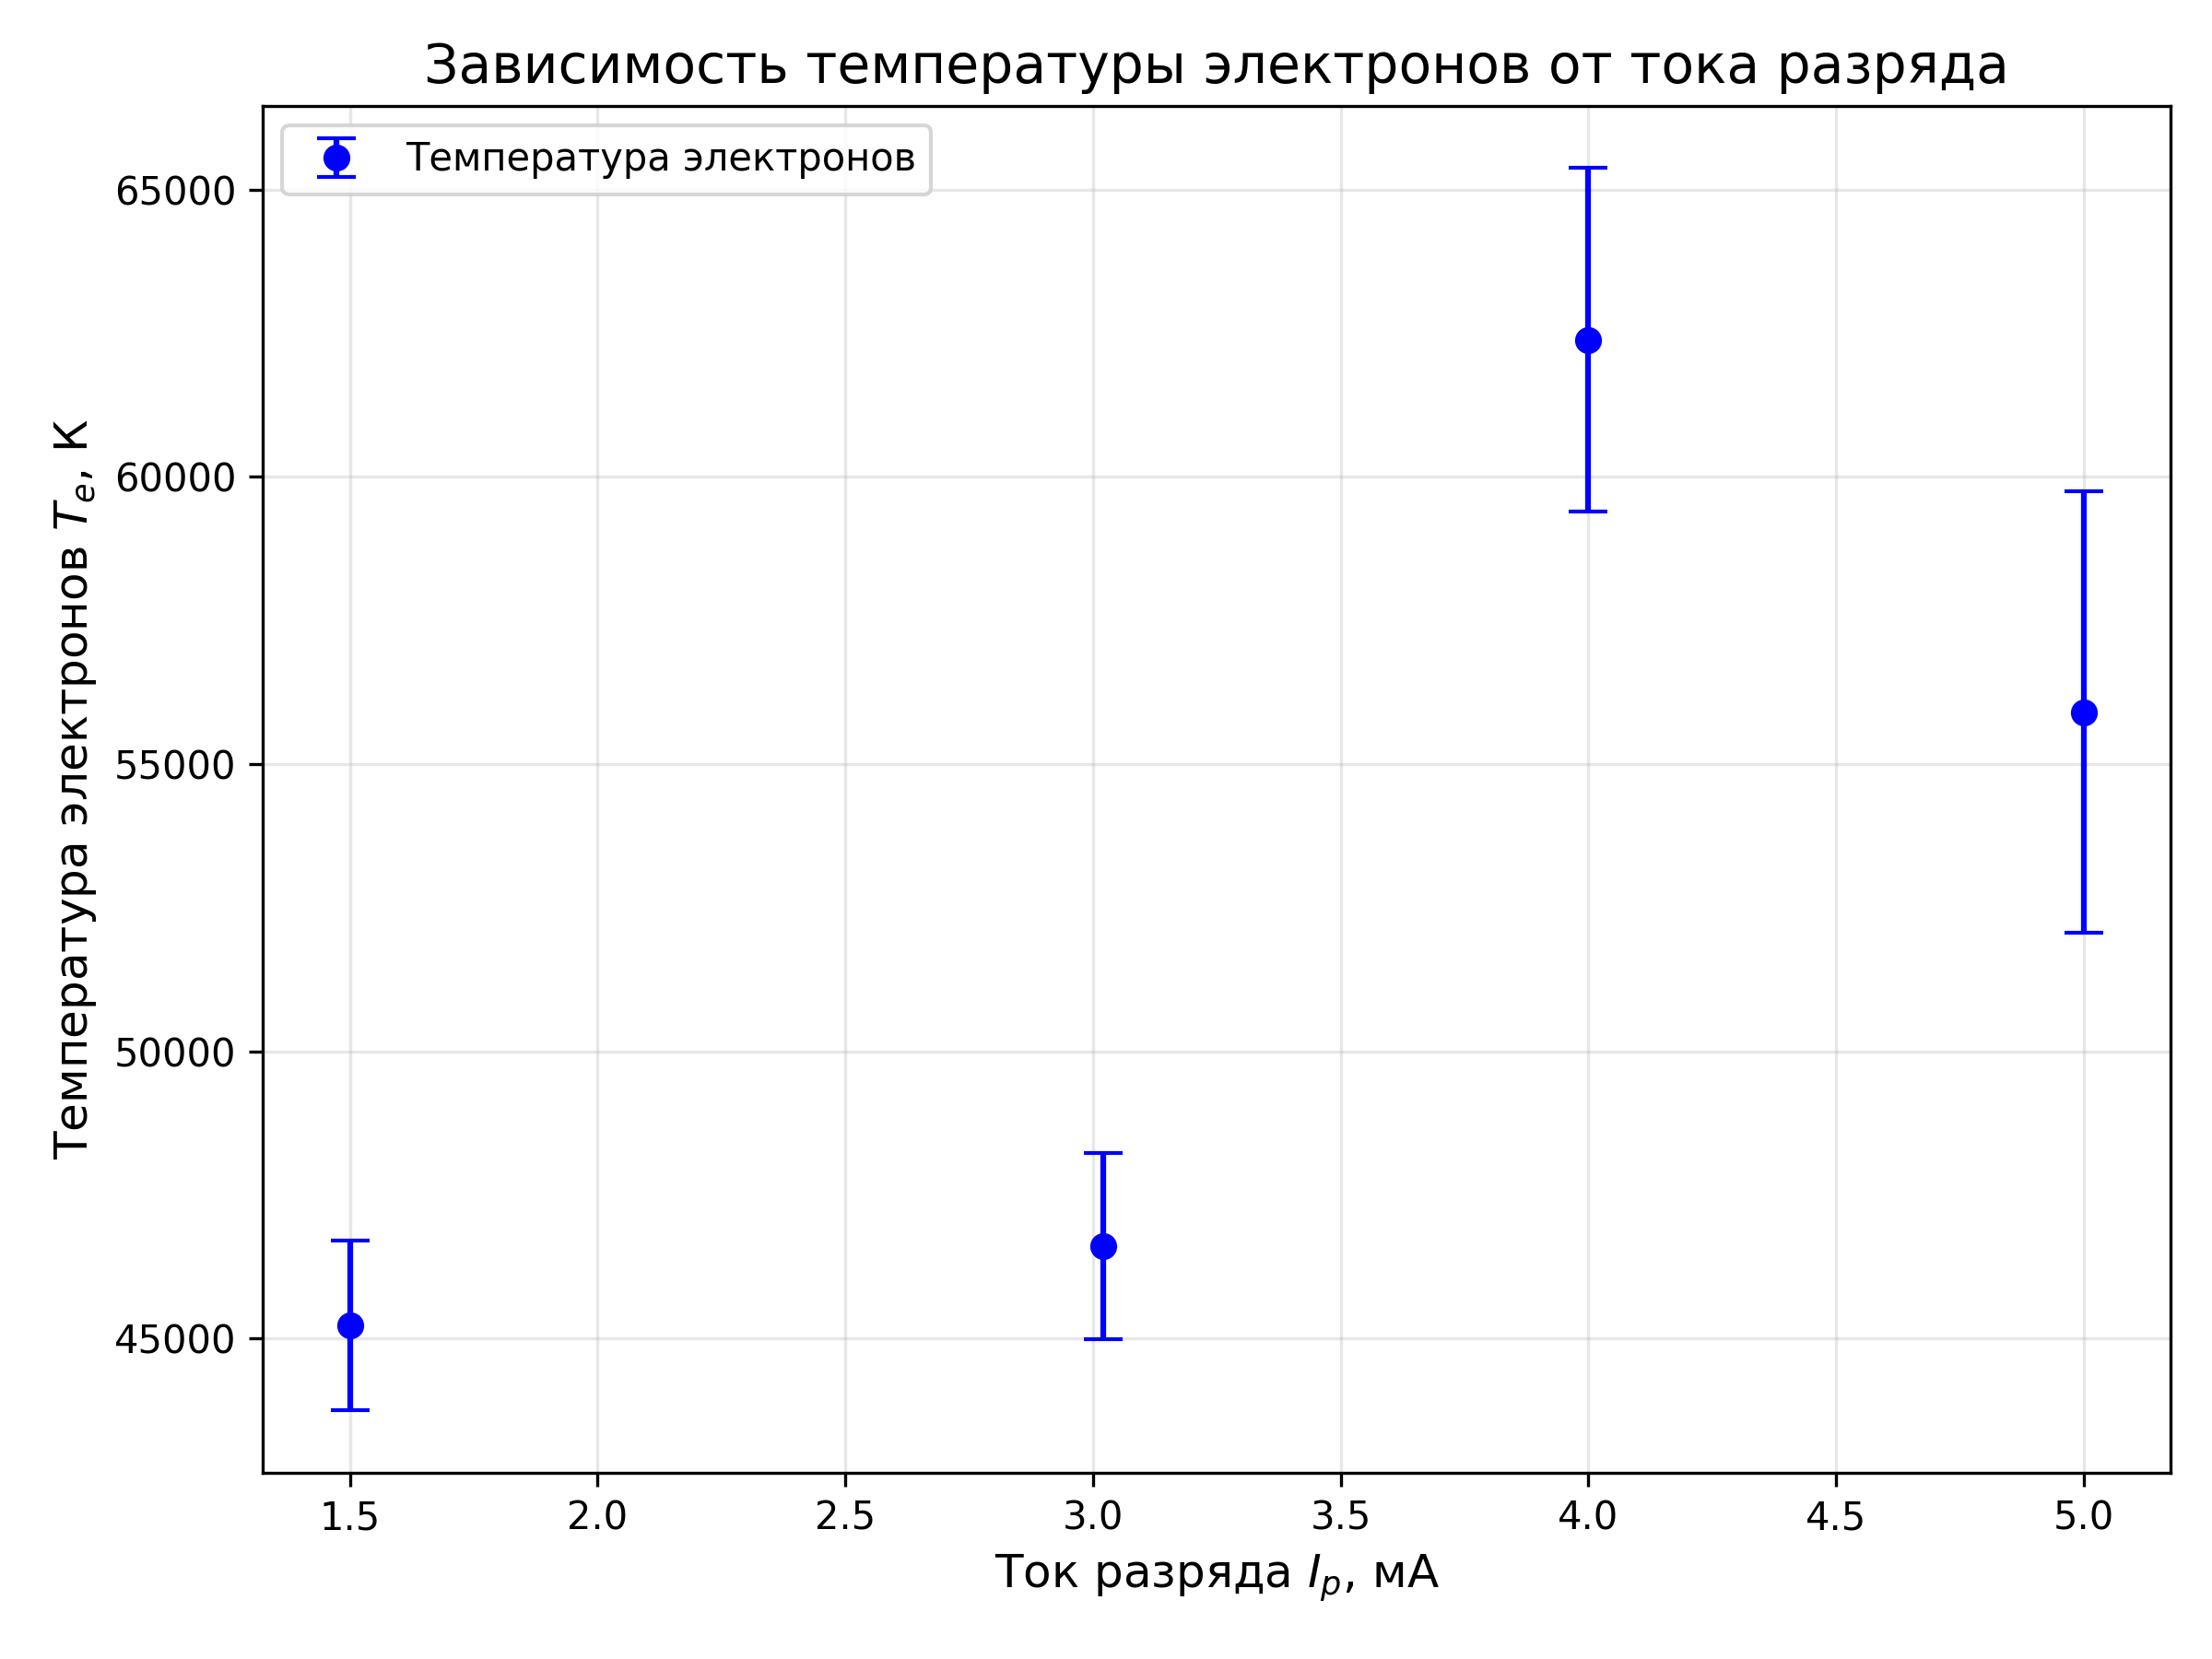
\includegraphics[width=0.7\textwidth]{Graphics/Te_vs_Ip_points.png}}
        \caption{График 4. Зависимость температуры электронов от тока разряда}
\end{figure}
\clearpage

Наклон прямой $n_e(I_\text{р})$ $k = (1,140 \pm 0,015) \cdot 10^{10} \ \frac{\text{см}^{-3}}{\text{мА}}$ ($\varepsilon_k = 1,35 \%$).
\end{enumerate}

\section{Результаты и обсуждения}

В данной работе было проведено исследование плазмы.
\begin{enumerate}
\item Построили ВАХ тлеющего разряда, по ней определили максимальное дифферециальное сопротивление $R_{\text{диф}}^{\text{ср}} = 93,8 \pm 6,9$ кОм ($\varepsilon_{R_{\text{диф}}^{\text{ср}}} = 7,36 \%$). Учитывая простоту метода определения этой величины, погрешность получилась удовлетворительной.
\item Построили ВАХ двойного зонда в плазме при разных токах рязряда. По ней получили разные характерные параметры плазмы (см. таблицу 3.). 
\item Наименьший характерный размер установки - это диаметр колбы $d = 0,2$ мм. Мы получили, что во всех случаях $r_D \ll d$, следовательно плазму можно считать квазинейтральной.
\item Для всех токов разряда получили, что степень ионизации $N_D \gg 1$ при давлении $P \approx 2$ торр, значит плазму разряда можно считать идеальной.
\item Исходя из теории $T_e$ слабо зависит от $I_\text{р}$, $I_\text{р} \sim n_e v_d$, где  $v_d$ - дрейфовая скорость, почти не зависит от тока и концентрации, следовательно $I_\text{р} \sim n_e$ - линейная зависимость. Исходя из построенных графиков 3 и 4 можно убедиться в этих соотношениях.
\end{enumerate}

\section{Результаты и обсуждения}

В ходе работы были исследованы параметры плазмы тлеющего газового разряда в неоне методом двойного зонда. По измеренным зондовым характеристикам при различных токах разряда определены температура и концентрация электронов, а также другие параметры плазмы, такие как дебаевский радиус и степень ионизации. Результаты показали, что плазма является слабо ионизованной и квазинейтральной, а с увеличением тока разряда температура электронов слабо изменяется, а их концентрация возрастает. Полученные данные согласуются с теоретическими представлениями о свойствах низкотемпературной неравновесной плазмы.
\end{document}